\chapter{Introduction}
The goal of this project is to develop a CNN capable of recognizing the presence of violence in the everyday CCTV footage in a binary detection system (violence/non violence). In the world of today it is fundamental for police and other forces to have a quick response in case of violent and criminal behavior especially when the people involved cannot dial the emergency lines due to immediate danger. The main idea it would be for these kind of AI algorithm to process enormous amount of video and signal it in case of foul play in real time. This project presented itself as a very difficult one due to the "\textit{dirtiness}" of the data-set used that, due to the fact the it was composed of real life CCTV footage, was not standardized, contained a lot o noise and many more other problems that will be explained in the next section.

\section{Dataset presentation}
The data-set was obtained by publicly available sources:
\begin{itemize}
	\item Smart-City CCTV Violence Detection Dataset\footnote{\url{https://www.kaggle.com/datasets/toluwaniaremu/smartcity-cctv-violence-detection-dataset-scvd/data}}: 1Gb
	\item seymanurakti/fight-detection-surv-dataset\footnote{\url{https://github.com/seymanurakti/fight-detection-surv-dataset}}: 100Mb
\end{itemize}

The first one was extracted from Kaggle and the data-set was divided into three sub-category (Non-Violence/Violence/Weapon-Violence)\footnote{Taken from version 2, now version 3 is available}, the second one was taken from a GitHub repository and the videos where divided into two sub folder (fight/noFight). The whole data-set was then divided by us into two main categories: violence and non-violence.

As previously said the problem, which is by itself quite difficult, was made harder due to the poor usability of the data-set that did not give any information on the videos aside form the category like: action frame and bounding boxes. Moreover the first set of videos received a usability score of 6.88 which represent a community rating of the data-set as a whole, for example some video contained writing in the screen, others were not CCTV footage, but live news one and some were recording through a phone of a screen with the footage. In addition the data-set was not standardized at all with videos with variable length and some greyscaled, some full color. Some example with the relative category are shown in Fig. \ref*{fig:overall}.

\begin{figure}[]
    \centering
    \begin{subfigure}{.5\textwidth}
        \centering
        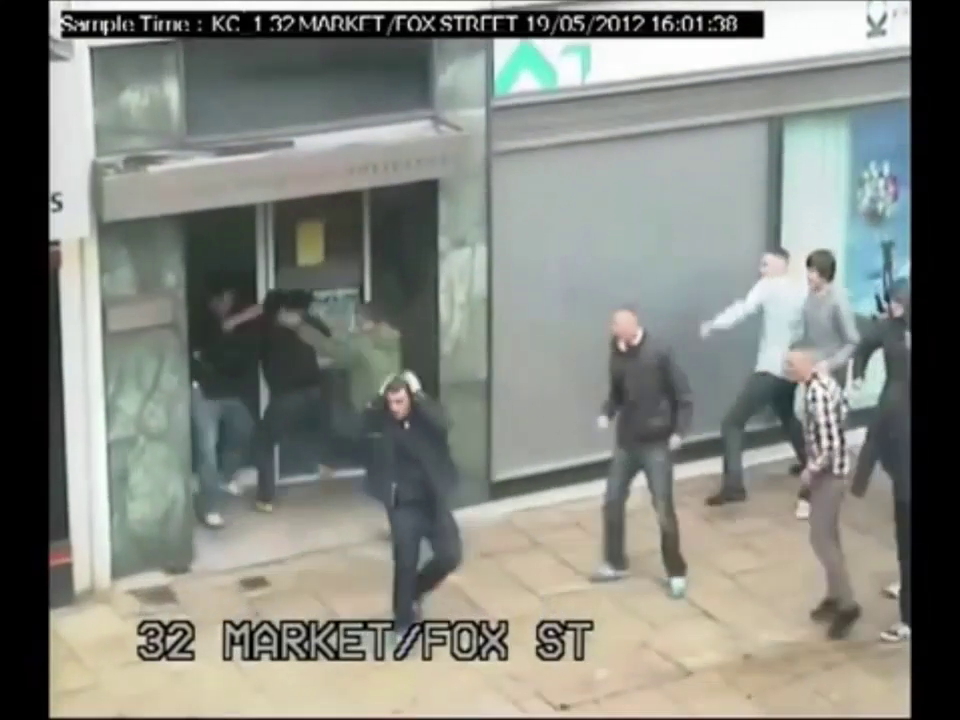
\includegraphics[width=\linewidth]{./images/V72-008.png}
        \caption{Image with non standardized size}
        \label{fig:sub1}
    \end{subfigure}%
    \begin{subfigure}{.5\textwidth}
        \centering
        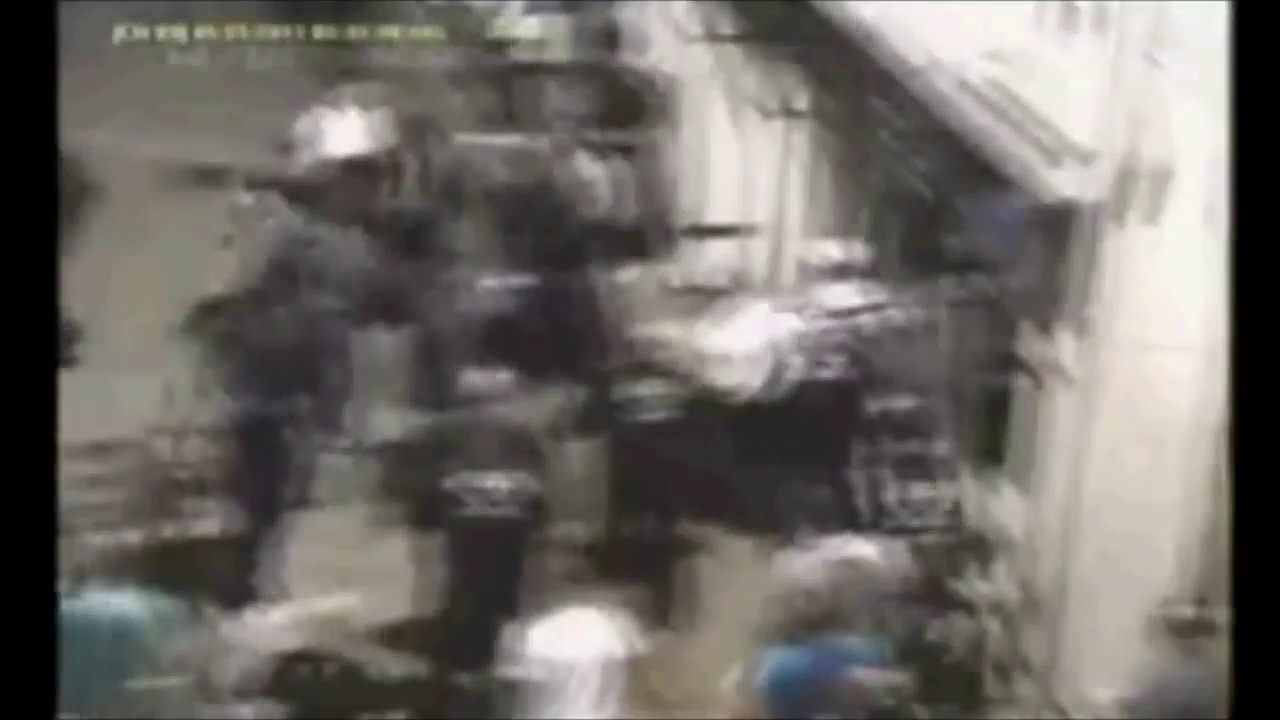
\includegraphics[width=\linewidth]{./images/V64-054.png}
        \caption{Image with blur and noise}
        \label{fig:sub2}
    \end{subfigure}\\
    \begin{subfigure}{.5\textwidth}
        \centering
        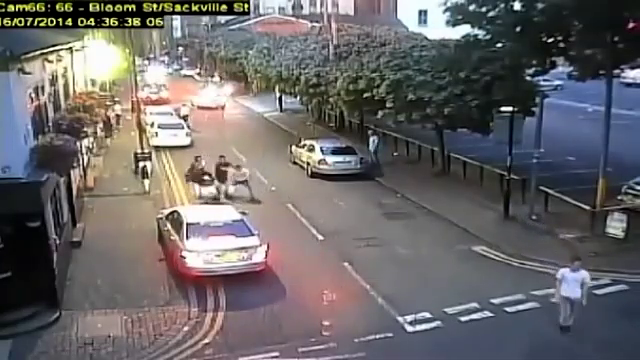
\includegraphics[width=\linewidth]{./images/V79-012.png}
        \caption{Violence in the distance}
        \label{fig:sub3}
    \end{subfigure}%
    \begin{subfigure}{.5\textwidth}
        \centering
        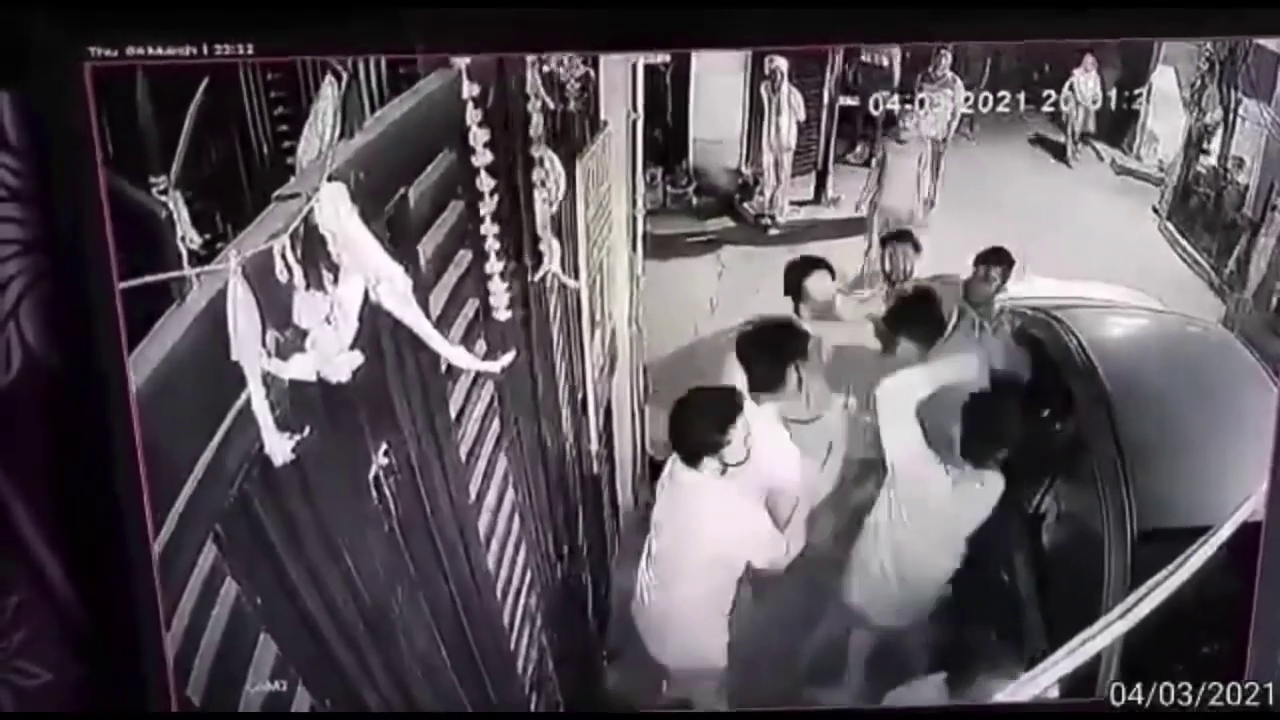
\includegraphics[width=\linewidth]{./images/V89-036.png}
        \caption{Violence close to camera}
        \label{fig:sub4}
    \end{subfigure}\\
    \begin{subfigure}{.5\textwidth}
        \centering
        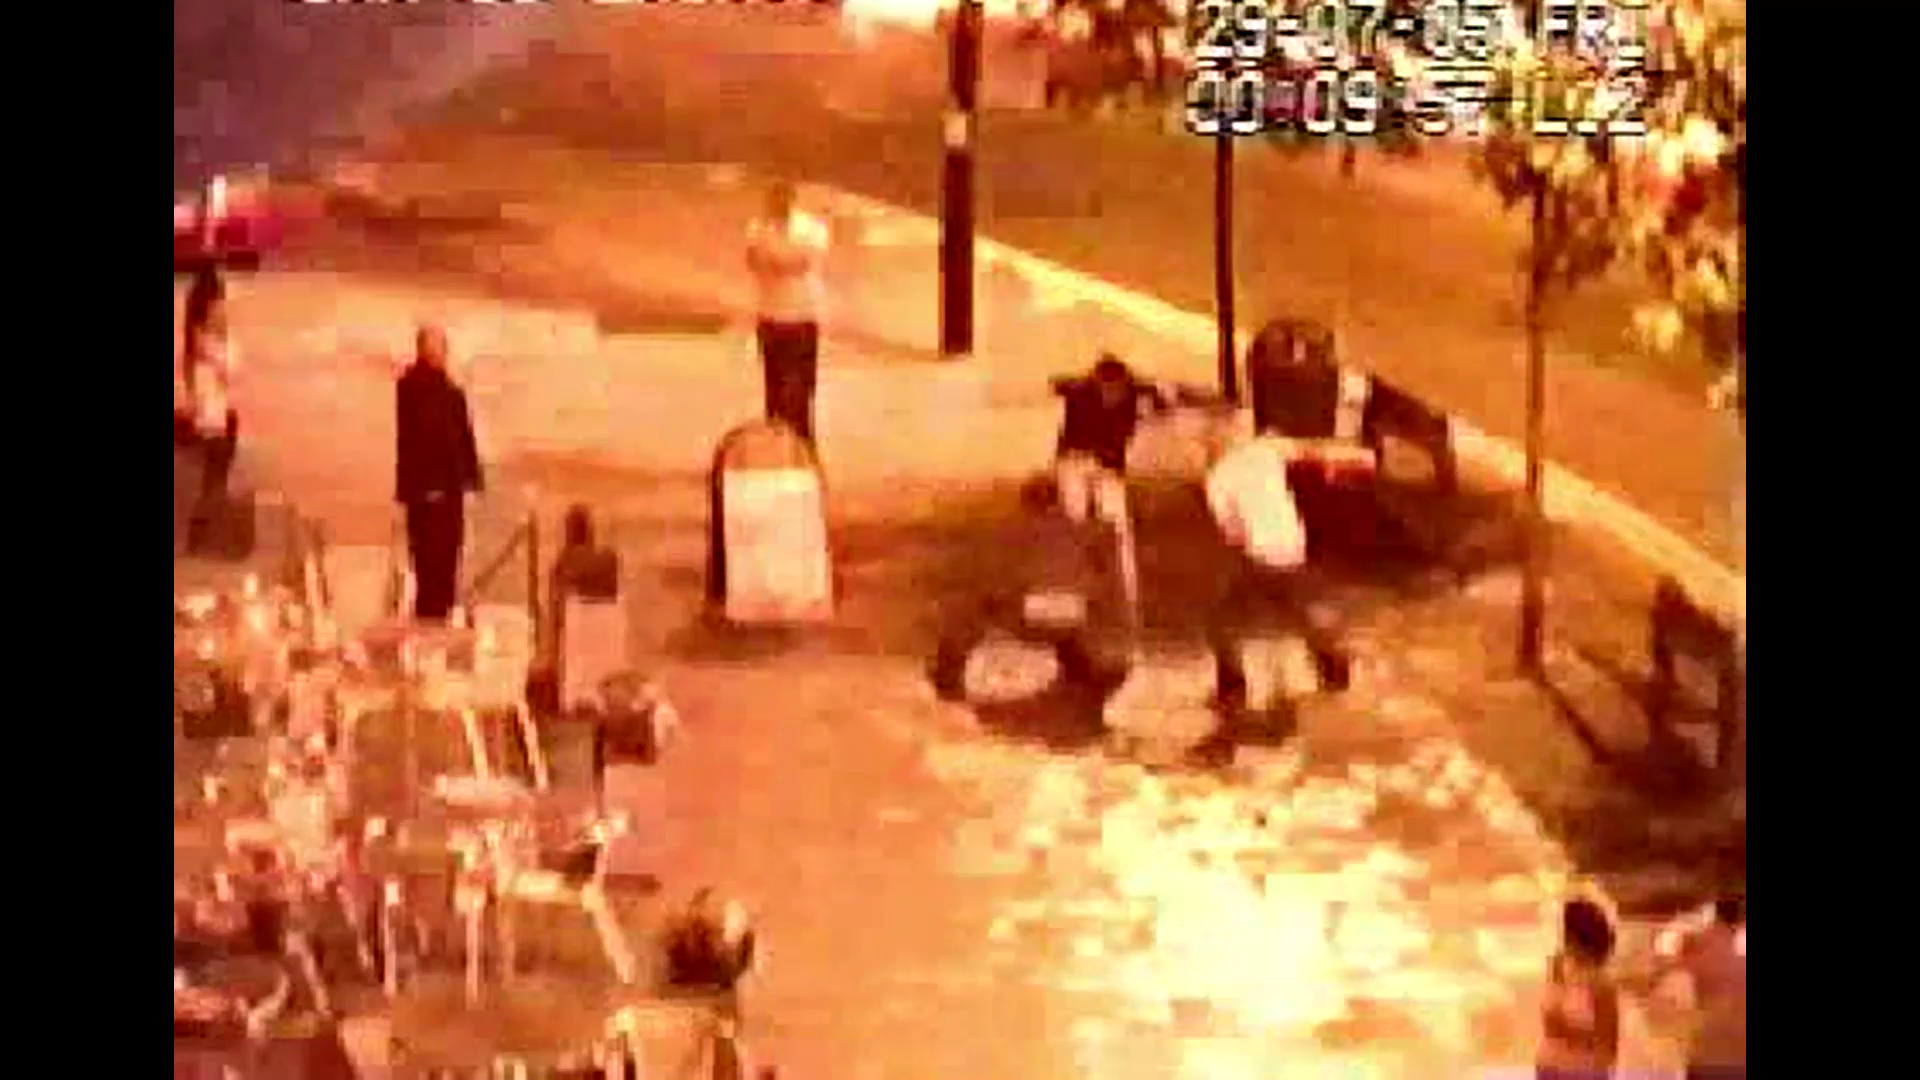
\includegraphics[width=\linewidth]{./images/V95-026.png}
        \caption{writing on the screen and brownscaled}
        \label{fig:sub5}
    \end{subfigure}%
    \begin{subfigure}{.5\textwidth}
        \centering
        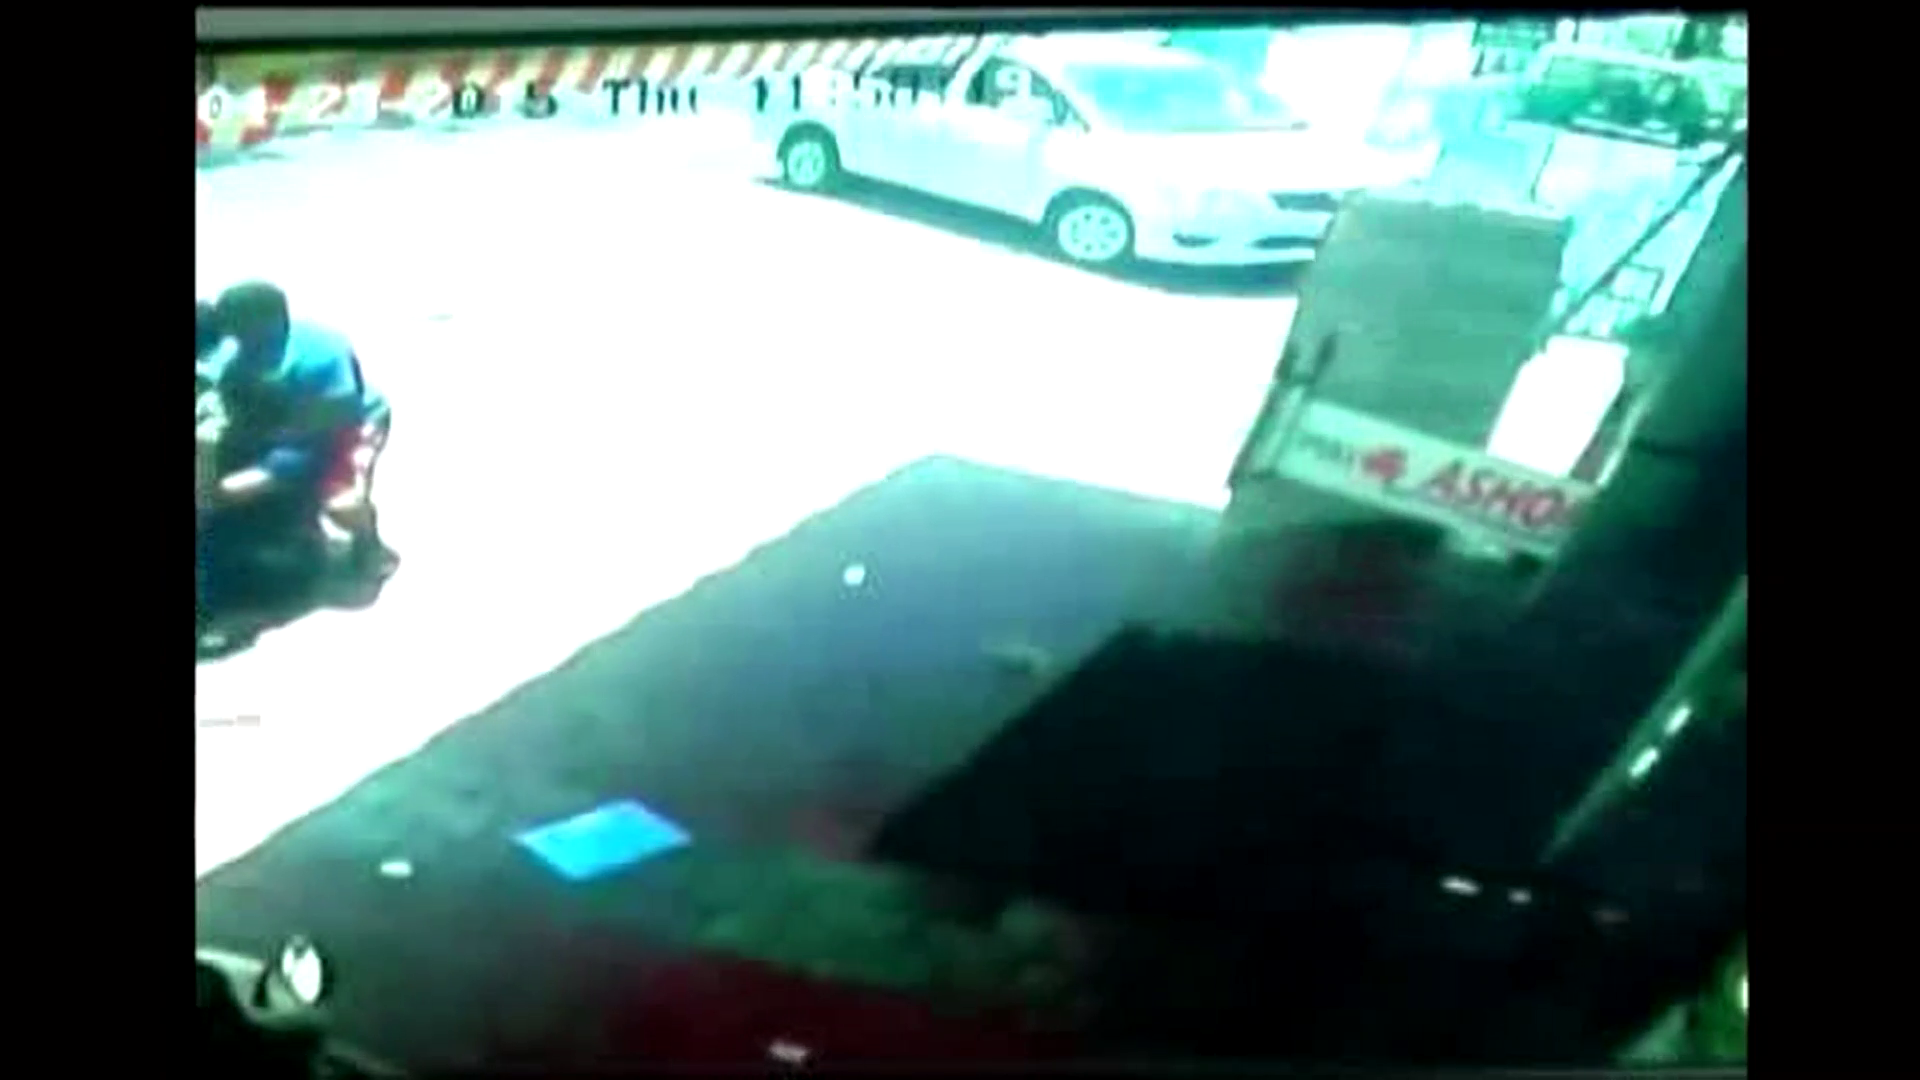
\includegraphics[width=\linewidth]{./images/V97-050.png}
        \caption{Violent frame with no violence}
        \label{fig:sub6}
    \end{subfigure}
    \caption{Some \textit{violent} frames from the data-set}
    \label{fig:overall}
\end{figure}

What these images prove is the dirtiness of the data-set and the difficulty of the task at hand. For example Fig \ref{fig:sub3} not only have violence in the distance, but also has writing on the screen, Fig \ref{fig:sub4} is a phone recoding of a desktop screen with the footage, Fig \ref{fig:sub6} is a frame with no violence at all, but it was classified as violent by the data-set because is part of a video that contains violence, but to remove all the frames that are not violent would have been too much of a hassle (more than 7k images to be process manually). In addition many videos like Fig. \ref{fig:sub2} and \ref{fig:sub4} are greyscaled. Others like Fig. \ref{fig:sub5} and \ref{fig:sub6} contains black bars on the side. This means that the data-set used was not standardized at all and there was no easy way to automatize the cleaning process.

\section{Goals and evaluation}
The goal of this project is to develop a CNN capable of recognizing the presence of violence in the everyday CCTV footage in a binary detection system. We wanted to evaluate our models with a real life approach, meaning that, although an high accuracy is desirable, it is not the only metric we are interested in, due to the differences in error cost between mislabelling violence as non violence and vice versa. In fact we are also interested in the precision and recall of the model, because we want to minimize the number of false negatives, meaning the case of violence not recognized as such, because it could result in damage of property or even a loss of life. So it is preferable to have a low false negative rate at the cost of a higher false positive rate without making it too high, causing the police to waste time and resources on false alarms. 